\documentclass{article}
\usepackage[utf8]{inputenc}
\usepackage{amsmath,amsthm,amssymb}
\usepackage{amsfonts}
\usepackage{arydshln}
\usepackage{enumitem}
\usepackage{float}
\usepackage{graphicx}
\usepackage{hyperref}
\usepackage{listings}
\usepackage{makecell}
\usepackage[margin=0.75in]{geometry}
\usepackage{multicol}
\usepackage{subcaption}
\usepackage{wrapfig}
\allowdisplaybreaks
\newtheorem{theorem}{Theorem}
\newtheorem{lemma}{Lemma}

\usepackage{fancyhdr}
\pagestyle{fancy}
\fancyhf{}
\fancyhead[L]{Bridgette Delight}
\fancyhead[C]{Math 465 - Homework 05 - \today}
\fancyhead[R]{\thepage}
\renewcommand{\headrulewidth}{2pt}

\title{{\large Math 465}\\ Homework 0X}
\author{Bridgette Delight}
\date{\today}

\begin{document}

\maketitle

\section{}
\begin{enumerate}[label = (\alph*)]
    \item  Construct the Lagrange interpolation polynomial $p_3 \in \mathcal{P}_3$ for the function
    \begin{equation*}
        f: x \to \sin(x) + \cos(x)
    \end{equation*}
    on the interval $[0, 1]$, with interpolation points $x_0 = 0$, $x_1 = 0.25$, $x_2 = 0.5$, and $x_3 = 1$. Present a figure showing $f(x)$ and $p_3(x)$ versus $x \in [0, 1]$.
    \item  Find an upper bound for the interpolation error on $[0, 1]$.
\end{enumerate}
\vspace{10mm}
%https://www.chegg.com/homework-help/questions-and-answers/construct-lagrange-interpolation-polynomial-p3-p3-function-f-x-sin-cosc-interval-0-1-inter-q42522942

\subsection*{(a)}

\begin{align*}
    x_0 = 0 \quad& f(x_0) = 1\\
    x_1 = 0.25 \quad& f(x_1) = 1.21631638\\
    x_2 = 0.5 \quad& f(x_2) = 1.3570081\\
    x_3 = 1 \quad& f(x_3) = 1.381773291\\
    f(x) &=  \frac{(x-0.25)(x-0.5)(x-1)}{(-0.25)(-0.75)(-1)}(1)
        +  \frac{(x-0)(x-0.5)(x-1)}{(0.25)(-0.75)(-1)}(1.21631638)+\\
        &  \frac{(x-0)(x-0.25)(x-1)}{(0.25)(0.75)(-1)}(1.35700081)
        +  \frac{(x-0)(x-0.25)(x-0.5)}{(0.25)(0.75)(1)}(1.381773291)\\
    f(x) &= 1 + 1.0066x - 0.545509 x^2 -0.0793181 x^3
\end{align*}

\begin{figure}[H]
    \centering
    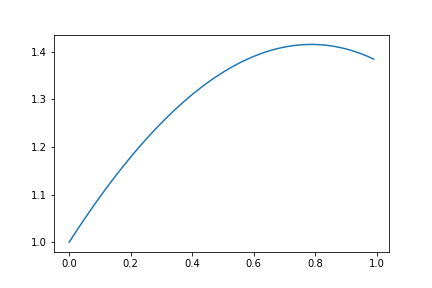
\includegraphics[width = .8 \linewidth]{images/hw05q01b.png}
    \caption{Caption}
    \label{fig:my_label}
\end{figure}

\subsection*{(b)}

\begin{align*}
    |F| &\le \frac{(0.5)^4}{4(4)}|F^4(x)| \le \frac{0.5^4}{16}\sqrt{2} = \sqrt{2}\\
    \text{Therefore, the upper bound is $\sqrt{2}$}\\
    f^4(x) &= \sin(x) + \cos(x) \le 1.414\\
\end{align*}


\section{}
Let $f: [-1,1] \to \mathbb{R}$ be continuous.
\begin{enumerate}[label = (\alph*)]
    \item Construct a Lagrange interpolation polynomial $p_1 \in P_1$ for $f$ using the interpolation points $x_0 = -1$ and $x_1 = 1$.
    \item Show further that if $f \in C^2([-1,1], \mathbb{R})$ then $$|f(x)-p_1(x)| \le \frac{M_2}{2}(1-x^2) \le \frac{M_2}{2},$$
    for all $x \in [-1,1]$, where $M_2 = \underset{x \in [-1,1]}{max} |f''(x)|$.
    \item Give an example of $f$, and a point $x$, for which
    $$|f(x)-p_1(x)|= \frac{M_2}{2}(1-x^2)$$
\end{enumerate}
\vspace{10mm}


\section{}
\begin{enumerate}[label = (\alph*)]
    \item Write down the Lagrange interpolation polynomial $p_1 \in \mathcal{P}_1$ for the function $f:x \to x^3$, using the points $x_0 = 0$, $x_1 = a$. Verify that Theorem 6.2 [Endre Suli and David Mayers, An Introduction to Numerical Analysis, Cambridge University Press, 2008] holds for this example by direct calculation, showing that in this case $\xi$ is unique and has the value $\xi=\frac{1}{3}(x+a)$.
    \item Repeat the calculation for the function $f: x \to (2x-a)^4$; show that in this case there are two possible values for $\xi$, and state their values.
\end{enumerate}
\vspace{10mm}


\section{}
 Given the distinct points $x_i$, $i = 0, 1,\dots, n + 1$, and the points $y_i$, $i = 0, 1, \dots , n + 1$, let $q$ be the Lagrange polynomial of degree $n$ for the set of points $\{(x_i, y_i) : i = 0, 1, \dots` , n\}$ and $r$ be the Lagrange polynomial of degree $n$ for the points $\{(x_i, y_i) : i = 1,\dots, n + 1\}$. Define
 \begin{equation*}
     p(x) = \frac{(x-x_0)r(x)-(x-x_{n+1}q(x))}{x_{n+1}-x_0}.
 \end{equation*}
 Show that $p$ is the Lagrange polynomial of degree $n+1$ for the points $\{(x_i,y_i): i =0,1,\dots, n+1 \}$.
\vspace{10mm}





\end{document}